
\subsection{Current Sources}\label{sec:currentsources}
The final stage of the Power-Mixing--DAC are the current sources. They provide a differential output over a 50$\Omega$ resistor. This setup is shown in Fig.\ref{figure:Current_sources}.
\begin{figure}[h!]
\begin{center}
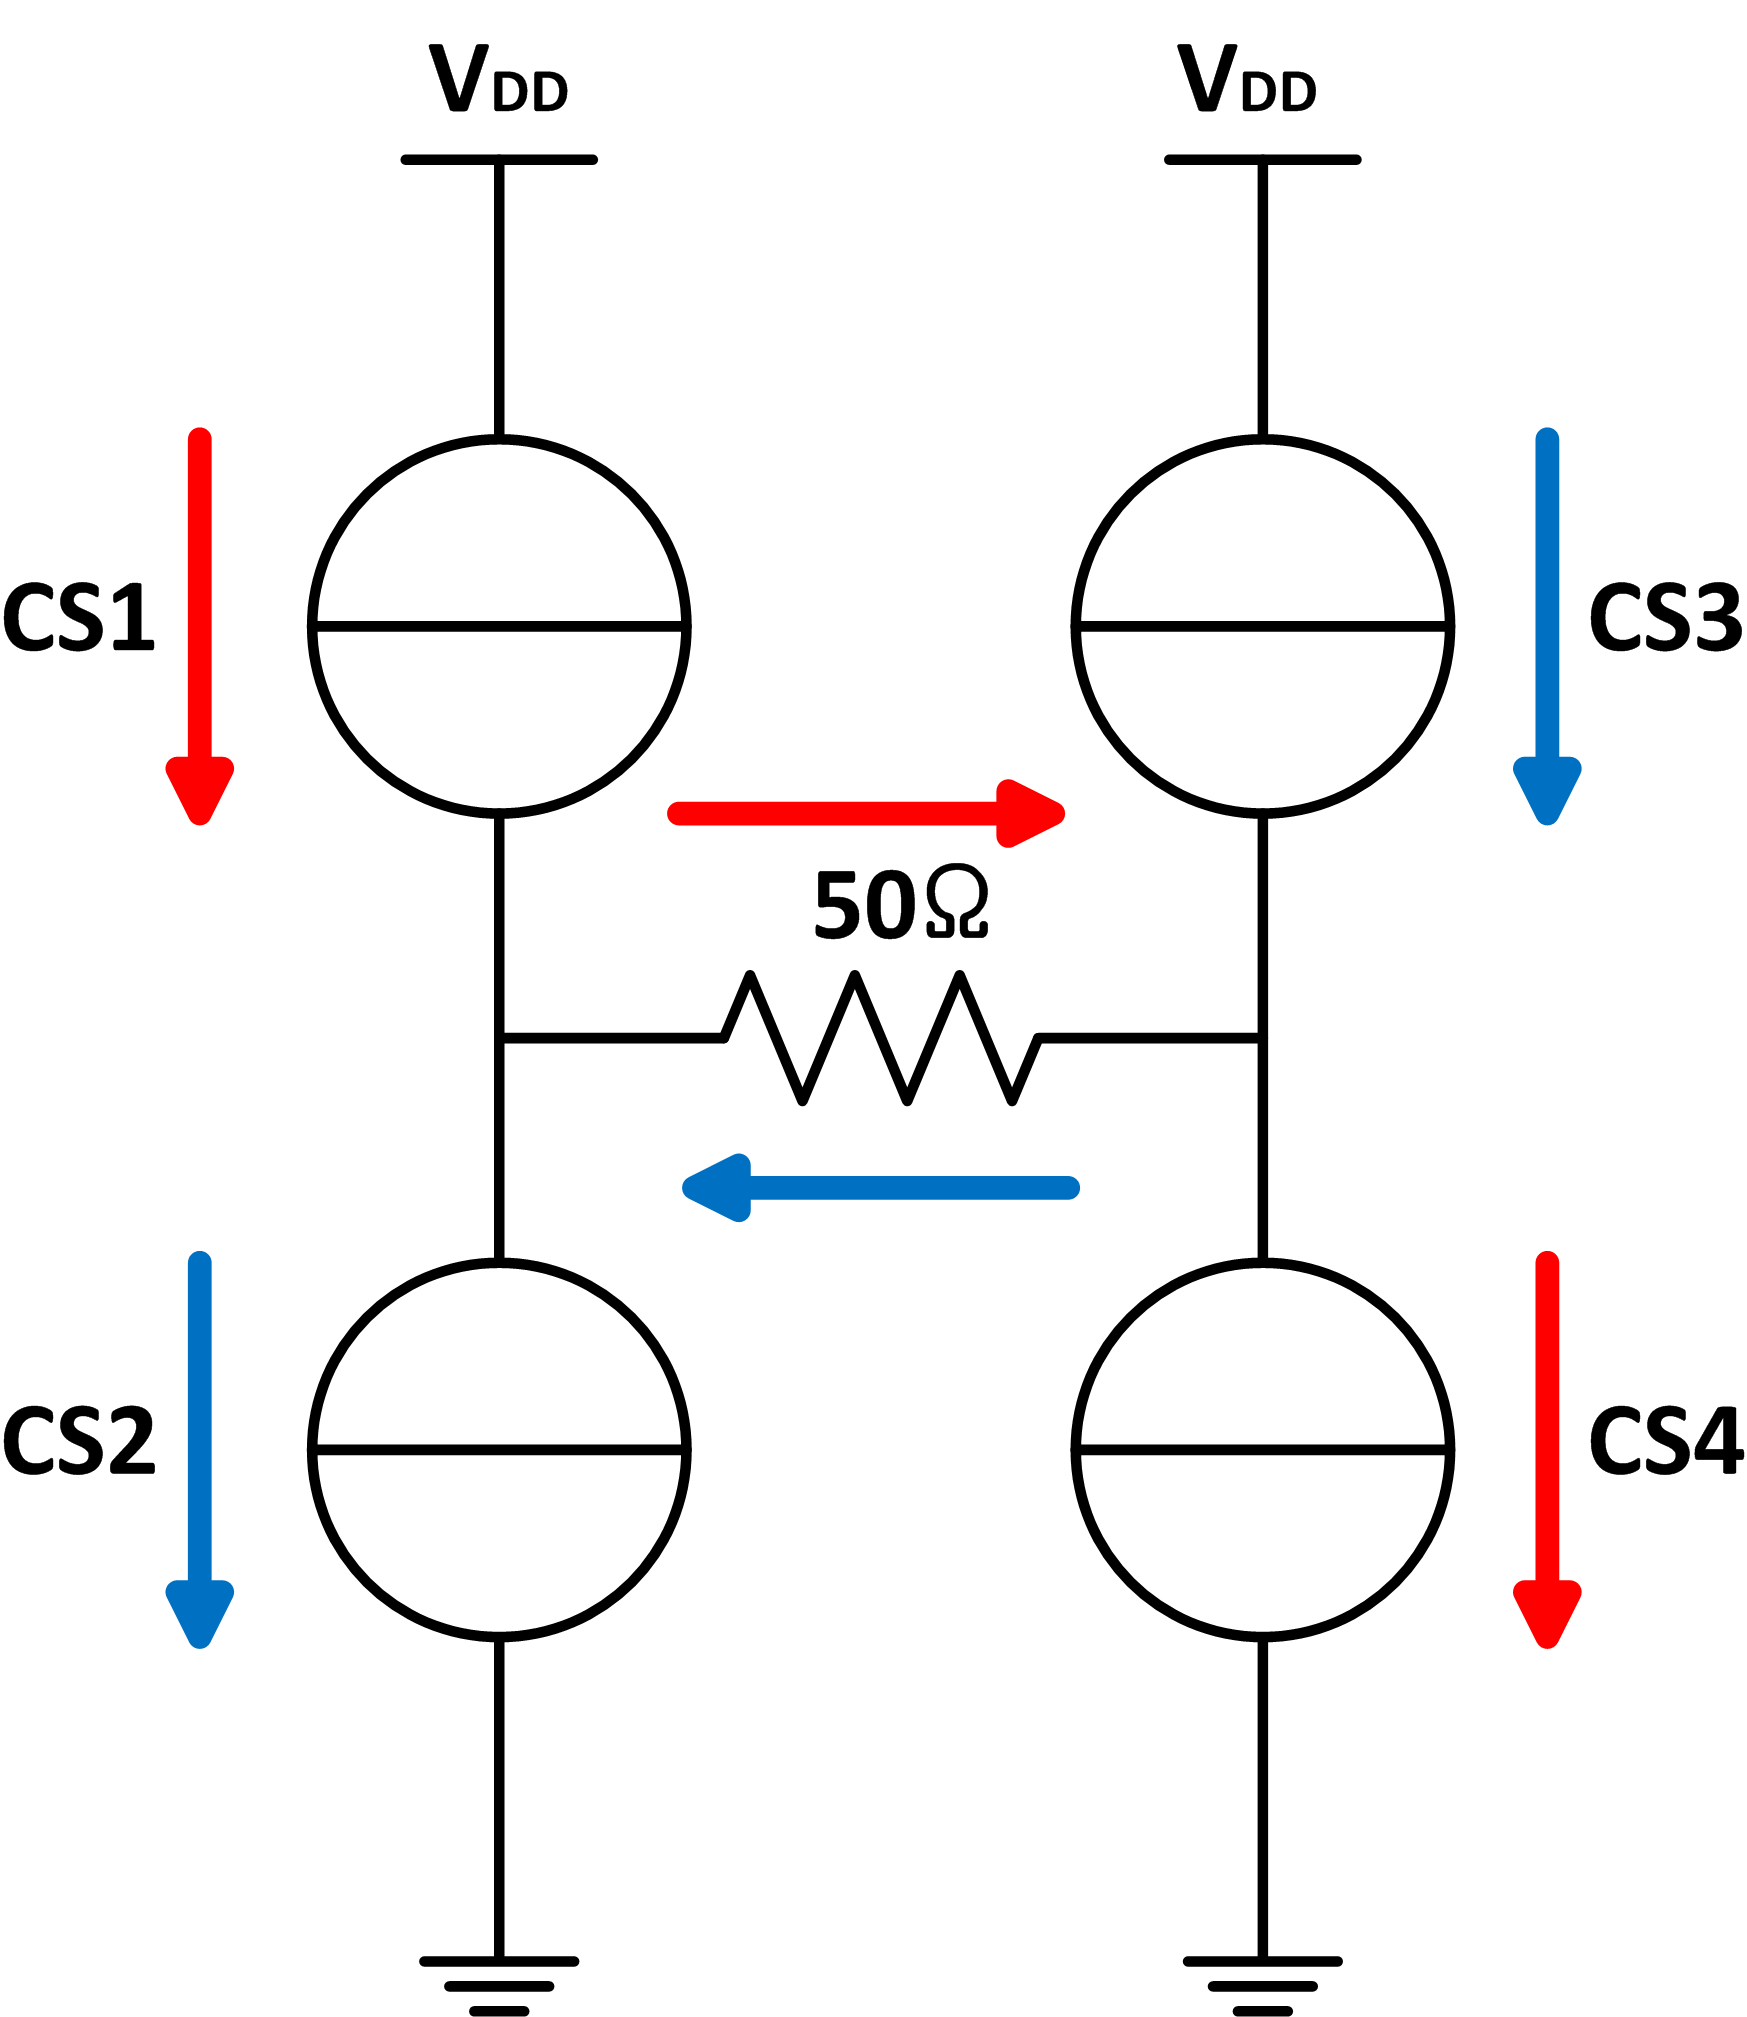
\includegraphics[width=0.3\textwidth]{CurrentSourceSchematic.png}
\caption{The final stage of the Power-Mixing--DAC: The current sources which will provide the differential output through the resistor.}
\label{figure:Current_sources}
\end{center}
\end{figure}
Due to the local oscillator, the current alternates between the path through CS1 and CS4 (see the red route in Fig.~\ref{figure:Current_sources}) and the the path through C3 and C2. (see the blue route in Fig.~\ref{figure:Current_sources}). 
The first design parameters are the supply volage and the switching devices. Because the DAC should be able to produce 50mA through a 50$\Omega$ resistor, the maximum voltage drop will be 2.5V. This already cancels out lower voltage supplies such as 1.2V and 2.5V. The resulting options are 3.3V and 5V. Because the stage consist of two current sources, the voltage headroom will be very limited in the 3.3V voltage supply. Therefore a 5V supply will be used as $V_{DD}$. This, along with the high switching speeds, limits the switching devices to the thick-oxide CMOS technology.\\
Due to the Power-Mixing- DAC design, the width and length of the CMOS are the only parameters. The most straightforward design method subscribes that the CMOS should always be in saturation so that the current through the CMOS is nearly independent, without channel-length modulation taken into account, of the drain-source voltage of the CMOS. This is directly related to the output impedance of the the switched current source. Therefore Eq.~\ref{eq:Overdrive} should be valid whatever the drain-source voltage.

\begin{equation}\label{eq:Overdrive}{V_{DS} > V_{ON} = V_{GS} - V_{TH}}\end{equation}

The drain-source voltage of both the NMOS and PMOS are minimal when the current through the resistor is maximal. In case of the NMOS this results in a minimum drain-source voltage of 1.25V. Because Eq.~\ref{eq:Overdrive} should be valid independent of the output, the maximum gate-source provided by the level shifter should be 1.95V, because the threshold voltage of the thick-oxide CMOS is 0.7V. Along with Eq.~\ref{eq:Drain current}, this provides a viable current sink.
\begin{equation}{I_D = \frac{1}{2}\mu_n C_{ox}\frac{W}{L}(V_{GS}-V_{TH})^2(1+\lambda V_{DS})}\label{eq:Drain current}\end{equation}
So by designing a current sink which operates at a $V_{GS}$ of 1.95V, the switching current sink will always be either in saturation or off. This provides a high output impedance and thus a high IMD3. Another advantage is the increase in efficiency.\\
For the PMOS the same design equations hold and thus they require a $V_{SG}$ of 1.95V to remain in saturation mode. So for the current source to provide current, the gate voltage should be witched between 3.05V (sourcing mode) and 5V (off mode).\\ 
The thick-oxide technology however, limits other parameters. The length of the thick-oxide CMOS transistor has as minimum of 200nm when the maximum available voltage headroom is 2.5V. In this configuration however, the maximum available voltage headroom needs to be minimal 2.5V. This limits the length of the transistor to a minimum of 300nm. Although a longer transistor has some advantages, such as a decrease in mismatch, it also mean a wider transistor to conduct the required current. A larger width however, results in higher input capacitance. To decrease the load on the level shifter, the length of both the PMOS ans the NMOS has been chosen to be optimized within the thick-oxide technology, i.e. 300nm.
The primary focus on each transistor is to make sure that it is able to handle the needed amount of current. As has been mentioned before, due to the channel-length modulation, M1 must be able to handle more current when the load is conducting 50mA as M15. Therefore every transistor has to be redesigned. The first transistor has been designed with the circuit found in Fig.\ref{fig:NMOS_Width_Sweep}. With this circuit a parametric sweep will be conducted to find the minimum width, to decrease the input capacitance of the transistor, to be able to conduct the required amount of current. This parametric sweep can be found in Fig.~\ref{fig:NMOS_Width_Sweep_Result}.
\begin{figure}[h]
\begin{center}
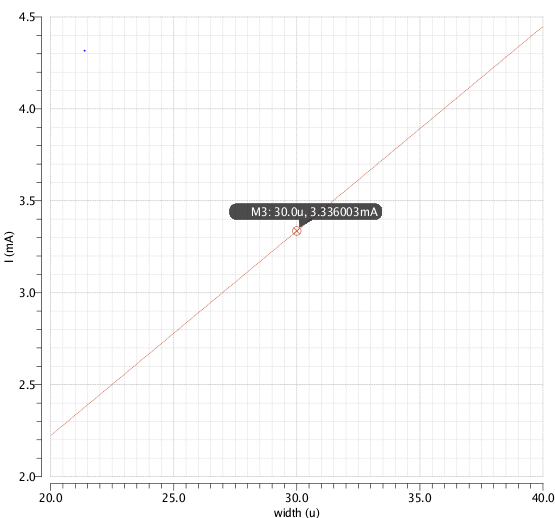
\includegraphics[width=0.4\textwidth]{NMOS_M1.png}
\caption{The current through the transistor versus its width. To make sure that the current through the transistor is 3.3mA, the width should be 10.96$\mu$m.}
\label{fig:NMOS_Width_Sweep_Result}
\end{center}
\end{figure}
So the width of the first NMOS should be 10.96$\mu$m to guarantee that it will sink 3.3mA when the $V_{GS}$ is 1.95V.\\
For the second transistor, a similar approach has been taken. Because the drain-source current will decrease, the current through M1 will increase. Therefore the second transistor is placed in parallel with M1, as it will be in the final design, and the width of the second transistor will be swept so that the transistors together will conduct 6.66mA. This technique will be repeated for each transistor. The list of all width and lengths of all NMOS thick-oxide transistors can be found in the appendix, table ~\ref{Tab:NMOS}.
The same technique has been used for the PMOS transistors. Due to the dummy technology, which was not able to simulate width over 100$\mu$m, each bit will be represented by two PMOS in parallel so that the width is maintained within the 100$\mu$m. This list can also be found in the appendix, table ~\ref{Tab:PMOS}.\\

When all of these transistors are designed in a single set-up, that is a setup as seen in Fig.~\ref{figure:Current_sources}, a sweep can be made through all bits. The results can be found in Fig.~\ref{fig:Final_result}. However, due to the switching and imperfections in both the NMOS and the PMOS, a error is present in the current. This error is signal dependent, as can be seen in Fig.\ref{fig:Current_error}.
\begin{figure}[h]
\begin{center}
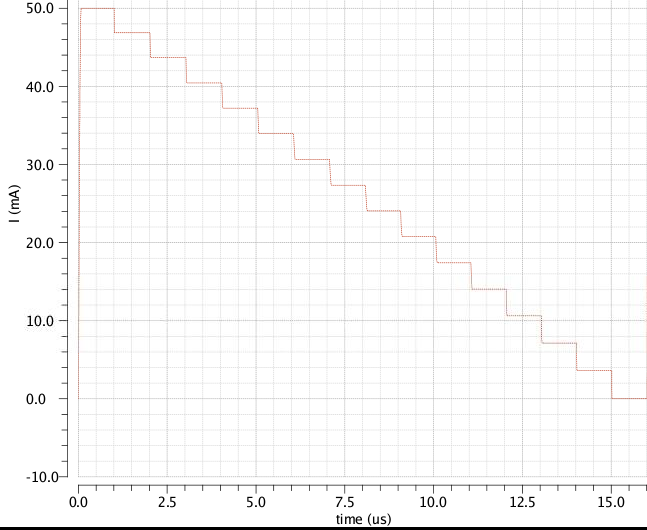
\includegraphics[width=0.4\textwidth]{Current_Cycle_Endstage.png}
\caption{A sweep through all possible currents, with a maximum of 50mA and a minimum of 0mA.}
\label{fig:Final_result}
\end{center}
\end{figure}
\begin{figure}[h]
\begin{center}
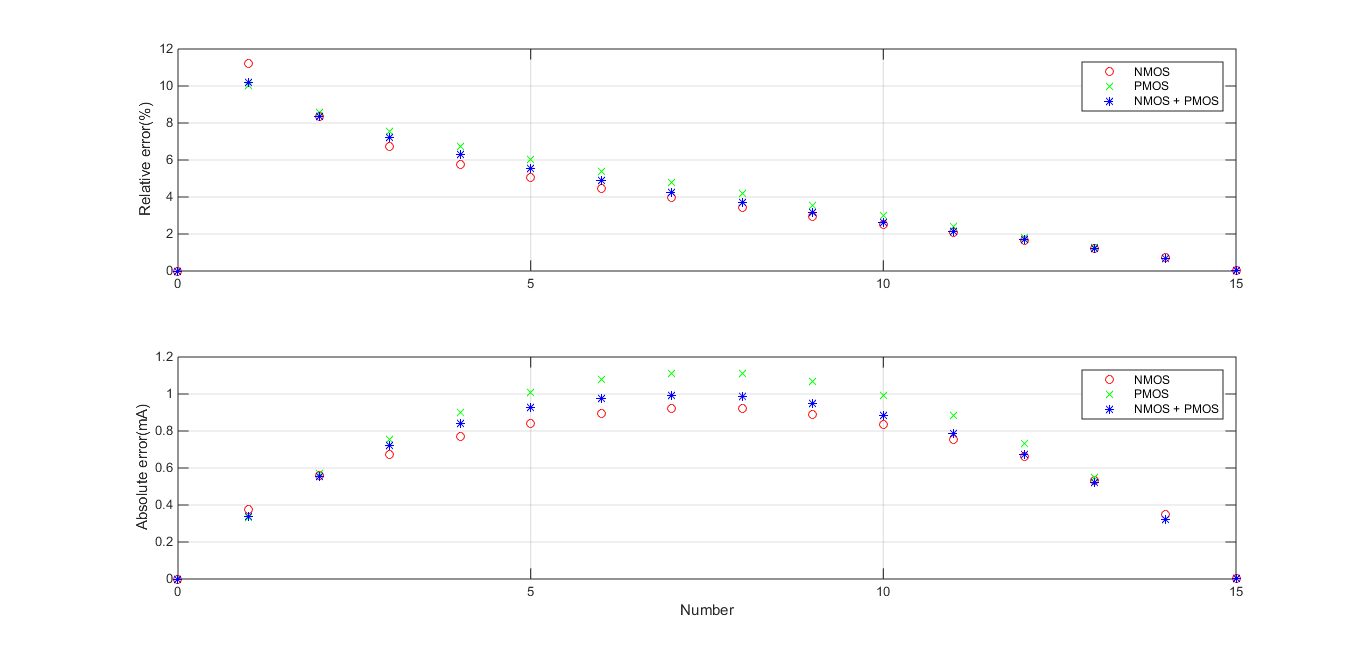
\includegraphics[width=\linewidth]{End_stage_errors.png}
\caption{The absolute and the relative current error in the endstage versus the input number of the DAC.}
\label{fig:Current_error}
\end{center}
\end{figure}

